\documentclass[aspectratio=169]{beamer}

\mode<presentation>
{
  \usetheme{Warsaw}
  % or ...

  \setbeamercovered{transparent}
  % or whatever (possibly just delete it)
}


\usepackage[english]{babel}
\usepackage[latin1]{inputenc}
\usepackage{graphicx}
\usepackage{amsmath,amsfonts,amssymb}

\setbeamertemplate{footline}[page number]

\newcommand{\pkg}{\textbf}
\newcommand{\code}{\texttt}


\title[Regular Expressions in R]{Regular Expressions in R}

\date{University of Minnesota\\April 26, 2013}



\begin{document}

\begin{frame}
  \titlepage
\end{frame}

\begin{frame}{Before We Begin}
Resources
\begin{itemize}
\item Slides at \url{http://github.com/rdpeng/Minnesota2013}
\item Lecture video on YouTube: \url{http://youtu.be/q8SzNKib5-4}
\item I am using R 3.0.0.
\end{itemize}
\end{frame}


\begin{frame}{Regular Expression Functions}
The primary R functions for dealing with regular expressions are
\begin{itemize}
\item \code{grep}, \code{grepl}: Search for matches of a regular
  expression/pattern in a character vector; either return the indices
  into the character vector that match, the strings that happen to
  match, or a TRUE/FALSE vector indicating which elements match
\item \code{regexpr}, \code{gregexpr}: Search a character vector for regular
  expression matches and return the indices of the string where the
  match begins and the length of the match
\item \code{sub}, \code{gsub}: Search a character vector for regular
  expression matches and replace that match with another string
\item \code{regexec}, \code{rematches}: Easier to explain through demonstration.
\end{itemize}
\end{frame}

\begin{frame}[fragile]{grep}
Here is an excerpt of the Baltimore City homicides dataset obtained from \url{http://data.baltimoresun.com/homicides/}
\begin{verbatim}
> homicides <- readLines("homicides.txt")
> homicides[1]
[1] "39.311024, -76.674227, iconHomicideShooting, 'p2', '<dl><dt>Leon 
Nelson</dt><dd class=\"address\">3400 Clifton Ave.<br />Baltimore, MD 
21216</dd><dd>black male, 17 years old</dd>
<dd>Found on January 1, 2007</dd><dd>Victim died at Shock 
Trauma</dd><dd>Cause: shooting</dd></dl>'"

> homicides[1000]
[1] "39.33626300000, -76.55553990000, icon_homicide_shooting, 'p1200',...
\end{verbatim}
How can I find the records for all the victims of shootings (as
opposed to other causes)?
\end{frame}

\begin{frame}[fragile]{grep}

\begin{verbatim}
> length(grep("iconHomicideShooting", homicides))
[1] 228
> length(grep("iconHomicideShooting|icon_homicide_shooting", homicides))
[1] 1003
> length(grep("Cause: shooting", homicides))
[1] 228
> length(grep("Cause: [Ss]hooting", homicides))
[1] 1003
> length(grep("[Ss]hooting", homicides))
[1] 1005
\end{verbatim}

\end{frame}


\begin{frame}[fragile]{grep}
\begin{verbatim}
> i <- grep("[cC]ause: [Ss]hooting", homicides)
> j <- grep("[Ss]hooting", homicides)
> str(i)
 int [1:1003] 1 2 6 7 8 9 10 11 12 13 ...
> str(j)
 int [1:1005] 1 2 6 7 8 9 10 11 12 13 ...
> setdiff(i, j)
integer(0)
> setdiff(j, i)
[1] 318 859
\end{verbatim}
\end{frame}


\begin{frame}[fragile]{grep}
\begin{verbatim}
> homicides[859]
[1] "39.33743900000, -76.66316500000, icon_homicide_bluntforce,
'p914', '<dl><dt><a href=\"http://essentials.baltimoresun.com/
micro_sun/homicides/victim/914/steven-harris\">Steven Harris</a>
</dt><dd class=\"address\">4200 Pimlico Road<br />Baltimore, MD 21215
</dd><dd>Race: Black<br />Gender: male<br />Age: 38 years old</dd>
<dd>Found on July 29, 2010</dd><dd>Victim died at Scene</dd>
<dd>Cause: Blunt Force</dd><dd class=\"popup-note\"><p>Harris was 
found dead July 22 and ruled a shooting victim; an autopsy
subsequently showed that he had not been shot,...</dd></dl>'"
\end{verbatim}
\end{frame}


\begin{frame}[fragile]{grep}
By default, \code{grep} returns the indices into the character vector
where the regex pattern matches. 
\begin{verbatim}
> grep("^New", state.name)
[1] 29 30 31 32
\end{verbatim}
Setting \code{value = TRUE} returns
the actual elements of the character vector that match.
\begin{verbatim}
> grep("^New", state.name, value = TRUE)
[1] "New Hampshire" "New Jersey"    "New Mexico"    "New York" 
\end{verbatim}
\code{grepl} returns a logical vector indicating which element matches.
\begin{verbatim}
> grepl("^New", state.name)
 [1] FALSE FALSE FALSE FALSE FALSE FALSE FALSE FALSE FALSE FALSE FALSE FALSE
[13] FALSE FALSE FALSE FALSE FALSE FALSE FALSE FALSE FALSE FALSE FALSE FALSE
[25] FALSE FALSE FALSE FALSE  TRUE  TRUE  TRUE  TRUE FALSE FALSE FALSE FALSE
[37] FALSE FALSE FALSE FALSE FALSE FALSE FALSE FALSE FALSE FALSE FALSE FALSE
[49] FALSE FALSE
\end{verbatim}
\end{frame}


\begin{frame}[fragile]{regexpr}
Some limitations of \code{grep}
\begin{itemize}
\item  The \code{grep} function tells you which strings in a character
  vector match a certain pattern but it doesn't tell you exactly where
  the match occurs or what the match is (for a more complicated
  regex). 
\item The \code{regexpr} function gives you the index into each string
  where the match begins and the length of the match for that string.
\item \code{regexpr} only gives you the first match of the string
  (reading left to right). \code{gregexpr} will give you all of the
  matches in a given string.
\end{itemize}
\end{frame}


\begin{frame}[fragile]{regexpr}
How can we find the date of the homicide?
\begin{verbatim}
> homicides[1]
[1] "39.311024, -76.674227, iconHomicideShooting, 'p2', '<dl><dt>Leon
Nelson</dt><dd class=\"address\">3400 Clifton Ave.<br />Baltimore, 
MD 21216</dd><dd>black male, 17 years old</dd>
<dd>Found on January 1, 2007</dd><dd>Victim died at Shock 
Trauma</dd><dd>Cause: shooting</dd></dl>'"
\end{verbatim}
Can we just 'grep' on ``Found''?
\end{frame}

\begin{frame}[fragile]{regexpr}
The word 'found' may be found elsewhere in the entry.
\begin{verbatim}
> homicides[954]
[1] "39.30677400000, -76.59891100000, icon_homicide_shooting, 'p816', 
'<dl><dd class=\"address\">1400 N Caroline St<br />Baltimore, MD 21213</dd>
<dd>Race: Black<br />Gender: male<br />Age: 29 years old</dd>
<dd>Found on March  3, 2010</dd><dd>Victim died at Scene</dd>
<dd>Cause: Shooting</dd><dd class=\"popup-note\"><p>Wheeler\\'s body 
was&nbsp;found on the grounds of Dr. Bernard Harris Sr.&nbsp;Elementary 
School</p></dd></dl>'"
\end{verbatim}
\end{frame}

\begin{frame}[fragile]{regexpr}
Let's use the pattern
\begin{verbatim}
<dd>[F|f]ound(.*)</dd>
\end{verbatim}
What does this look for?
\begin{verbatim}
> regexpr("<dd>[F|f]ound(.*)</dd>", homicides[1:10])
 [1] 177 178 188 189 178 182 178 187 182 183
attr(,"match.length")
 [1] 93 86 89 90 89 84 85 84 88 84
attr(,"useBytes")
[1] TRUE
> substr(homicides[1], 177, 177 + 93 - 1)
[1] "<dd>Found on January 1, 2007</dd><dd>Victim died at Shock
 Trauma</dd><dd>Cause: shooting</dd>"
\end{verbatim}
\end{frame}


\begin{frame}[fragile]{regexpr}
The previous pattern was too greedy and matched too much of the
string. We need to use the \code{?} metacharacter to make the regex
``lazy''.
\begin{verbatim}
> regexpr("<dd>[F|f]ound(.*?)</dd>", homicides[1:10])
 [1] 177 178 188 189 178 182 178 187 182 183
attr(,"match.length")
 [1] 33 33 33 33 33 33 33 33 33 33
attr(,"useBytes")
[1] TRUE

> substr(homicides[1], 177, 177 + 33 - 1)
[1] "<dd>Found on January 1, 2007</dd>"

\end{verbatim}
\end{frame}

\begin{frame}[fragile]{regmatches}
One handy function is \code{regmatches} which extracts the matches in
the strings for you without you having to use \code{substr}.
\begin{verbatim}
> r <- regexpr("<dd>[F|f]ound(.*?)</dd>", homicides[1:5])
> regmatches(homicides[1:5], r)
[1] "<dd>Found on January 1, 2007</dd>" "<dd>Found on January 2, 2007</dd>"
[3] "<dd>Found on January 2, 2007</dd>" "<dd>Found on January 3, 2007</dd>"
[5] "<dd>Found on January 5, 2007</dd>"
\end{verbatim}
\end{frame}

\begin{frame}[fragile]{sub/gsub}
Sometimes we need to clean things up or modify strings by matching a
pattern and replacing it with something else. For example, how can we
extract the data from this string?
\begin{verbatim}
> x <- substr(homicides[1], 177, 177 + 33 - 1)
> x
[1] "<dd>Found on January 1, 2007</dd>"
\end{verbatim}
We want to strip out the stuff surrounding the ``January 1, 2007''
piece.
\begin{verbatim}
> sub("<dd>[F|f]ound on |</dd>", "", x)
[1] "January 1, 2007</dd>"

> gsub("<dd>[F|f]ound on |</dd>", "", x)
[1] "January 1, 2007"
\end{verbatim}
\end{frame}


\begin{frame}[fragile]{sub/gsub}
sub/gsub can take vector arguments
\begin{verbatim}
> r <- regexpr("<dd>[F|f]ound(.*?)</dd>", homicides[1:5])
> m <- regmatches(homicides[1:5], r)
> m
[1] "<dd>Found on January 1, 2007</dd>" "<dd>Found on January 2, 2007</dd>"
[3] "<dd>Found on January 2, 2007</dd>" "<dd>Found on January 3, 2007</dd>"
[5] "<dd>Found on January 5, 2007</dd>"
> d <- gsub("<dd>[F|f]ound on |</dd>", "", m)
[1] "January 1, 2007" "January 2, 2007" "January 2, 2007" "January 3, 2007"
[5] "January 5, 2007"
> as.Date(d, "%B %d, %Y")
[1] "2007-01-01" "2007-01-02" "2007-01-02" "2007-01-03" "2007-01-05"
\end{verbatim}
\end{frame}

\begin{frame}[fragile]{regexec}
The \code{regexec} function works like \code{regexpr} except it gives
you the indices for parenthesized sub-expressions.
\begin{verbatim}
> regexec("<dd>[F|f]ound on (.*?)</dd>", homicides[1])
[[1]]
[1] 177 190
attr(,"match.length")
[1] 33 15

> regexec("<dd>[F|f]ound on .*?</dd>", homicides[1])
[[1]]
[1] 177
attr(,"match.length")
[1] 33
\end{verbatim}
\end{frame}


\begin{frame}[fragile]{regexec}
  Now we can extract the string in the parenthesized sub-expression.
\begin{verbatim}
> regexec("<dd>[F|f]ound on (.*?)</dd>", homicides[1])
[[1]]
[1] 177 190
attr(,"match.length")
[1] 33 15

> substr(homicides[1], 177, 177 + 33 - 1)
[1] "<dd>Found on January 1, 2007</dd>"

> substr(homicides[1], 190, 190 + 15 - 1)
[1] "January 1, 2007"
\end{verbatim}
\end{frame}

\begin{frame}[fragile]{regexec}
Even easier with the \code{regmatches} function.
\begin{verbatim}
> r <- regexec("<dd>[F|f]ound on (.*?)</dd>", homicides[1:2])
> regmatches(homicides[1:2], r)
[[1]]
[1] "<dd>Found on January 1, 2007</dd>" "January 1, 2007"                  

[[2]]
[1] "<dd>Found on January 2, 2007</dd>" "January 2, 2007"
\end{verbatim}
\end{frame}

\begin{frame}[fragile]{regexec}
\begin{verbatim}
> homicides[1]
[1] "39.311024, -76.674227, iconHomicideShooting, 'p2', '<dl><dt>Leon 
Nelson</dt><dd class=\"address\">3400 Clifton Ave.<br />Baltimore, MD 
21216</dd><dd>black male, 17 years old</dd>
<dd>Found on January 1, 2007</dd><dd>Victim died at Shock 
Trauma</dd><dd>Cause: shooting</dd></dl>'"
\end{verbatim}
Let's make a plot of monthly homicide counts
\begin{verbatim}
> r <- regexec("<dd>[F|f]ound on (.*?)</dd>", homicides)
> m <- regmatches(homicides, r)
> dates <- sapply(m, function(x) x[2])
> dates <- as.Date(dates, "%B %d, %Y")
> hist(dates, "month", freq = TRUE)
\end{verbatim}
\end{frame}

\begin{frame}[fragile]{regexec}
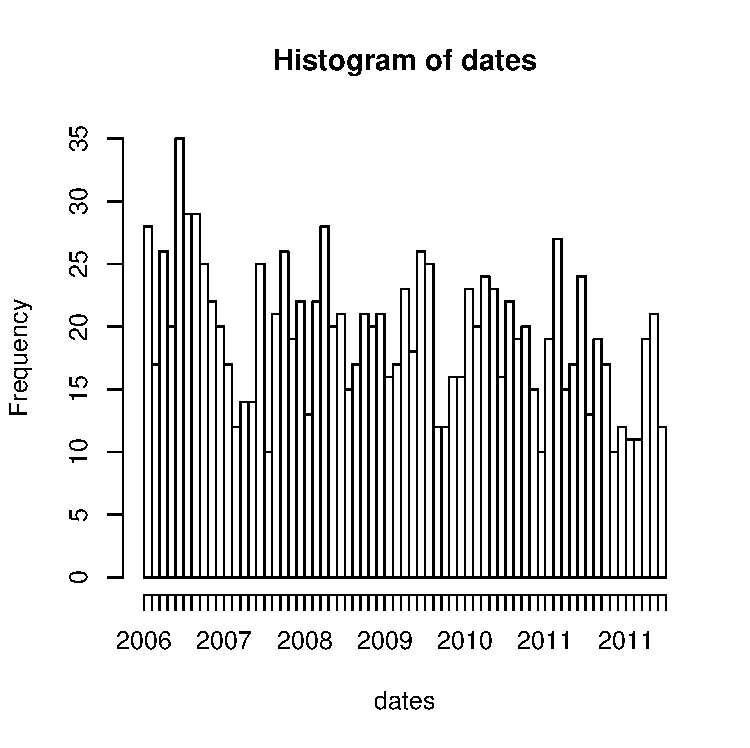
\includegraphics[height=3.2in]{homicide-month}
\end{frame}


\begin{frame}{Summary}
The primary R functions for dealing with regular expressions are
\begin{itemize}
\item \code{grep}, \code{grepl}: Search for matches of a regular
  expression/pattern in a character vector
\item \code{regexpr}, \code{gregexpr}: Search a character vector for regular
  expression matches and return the indices where the match begins;
  useful in conjunction with \code{regmatches}
\item \code{sub}, \code{gsub}: Search a character vector for regular
  expression matches and replace that match with another string
\item \code{regexec}, \code{rematches}: Gives you indices of parethensized sub-expressions.
\end{itemize}
\end{frame}








\end{document}
